
% Software Sustainability Challenge submission should be no more than
% 2-pages long, and use the ACM sigconf template (for more details,
% see the main conference Call For Papers). They will be peer
% reviewed, and accepted submissions will be presented at the
% conference as either part of a panel or lightning talk and/or within
% a poster session (as determined by the Programme Chair). Challenge
% submissions will not be included in the main DLfM proceedings, but
% will be published on the conference website; they will additionally
% be used (with appropriate credit given) to inform a report into
% Digital Musicology for the UK Software Sustainability Institute.
%
% Challenge contributions must be submitted via the DLfM 2023
% EasyChair page by Friday 29 September.

\documentclass[sigconf, nonacm=true]{acmart}
%\documentclass[sigconf, nonacm=true, authordraft=true, anonymous=true]{acmart}
\setcopyright{none}

\begin{document}
\title{Software Sustainability Challenge: ECOLM and Lute Tablature}

\acmConference[DLfM'23]{10th International Conference on Digital Libraries for Musicology}{November 10, 2023}{Milan, Italy}

\author{Chris Cannam}
\orcid{https://orcid.org/0009-0001-9814-6512}
\affiliation{%
  \institution{Particular Programs Ltd}
  \city{London}
  \country{UK}}
\email{chris.cannam@particularprograms.co.uk}

\author{David Lewis}
\affiliation{%
  \institution{Goldsmiths, University of London}
  \city{London}
  \country{UK}}
\email{d.lewis@gold.ac.uk}

\author{Tim Crawford}
\affiliation{%
  \institution{Goldsmiths, University of London}
  \city{London}
  \country{UK}}
\email{t.crawford@gold.ac.uk}

\maketitle
\begin{sloppypar}

  % Authors should use headings from the following list to structure
  % their submissions, addressing implications for sustainability in all
  % relevant sections, and using as many as are applicable for their
  % scenario:
  %
  % ·       Nature and purpose of the sustainable tool or resource
  % - Yes
  %
  % ·       Audience and users, disciplines and subjects
  % - Yes
  %
  % ·       Position within the research lifecycle
  % - Possibly not
  %
  % ·       Means of access and accessibility
  % - Possibly not
  %
  % ·       Current and future requirements, or implementations
  % - Yes
  %
  % ·       Challenges for sustainability
  % - Yes, especially
  %
  % ·       Future directions
  % - Yes, tentatively

  \section{Nature and purpose of the sustainable tool or resource}

  {\bf ECOLM} or ``Electronic Corpus of Lute Music'' (1999-2002) was a
  project led by Tim Crawford at King's College London which developed
  and populated a database of lute tablature encodings with metadata,
  for scholarly use, queried using a web interface. Subsequent
  projects {\bf ECOLM II} (2002-2006) and {\bf ECOLM III} (2012)
  expanded the database and used it for some computational
  musicological investigations. The resulting database was hosted on a
  public-facing web server at Goldsmiths, University of
  London.\footnote{http://doc.gold.ac.uk/isms/ecolm/database/} It is
  still running today, although nobody is formally responsible for
  maintaining it.

  ECOLM is a relatively small scholarly resource with around 2,000
  carefully-curated encodings. A number of other public lute tablature
  resources exist, of varying size, quality, and consistency (see
  section \ref{audience}). These typically face challenges to
  sustainability similar to those of ECOLM (see section
  \ref{challenges}). It seems useful to consider those challenges for
  such resources together, at least insofar as they share an
  audience.

  Lute tablature is of unusual interest as a field because it is
  poorly handled by existing digital musical resources even though it
  is not intrinsically obscure or esoteric. It is a straightforward
  notation that was among the most accessible media for music
  distribution in Europe from the late 15th to the early 18th century,
  so is far more historically significant than its representation in
  the digital world might suggest.
  
  \section{Audience and users, disciplines and subjects}\label{audience}

  We are considering here the sustainability of at least five lute
  tablature datasets: ECOLM itself; {\bf
    lutemusic.org}\footnote{https://lutemusic.org/} by Sarge Gerbode;
  {\bf mss.slweiss.de}\footnote{https://mss.slweiss.de/} curated by
  Peter Steur and the late Markus Lutz; a set of scans from {\bf Lute
    Society publications} curated by John Robinson; and a set of
  transcriptions of {\bf editions by Pierre Phal\`ese} curated by Jan
  Burgers. All of these are either Creative Commons licensed or have
  been offered by their maintainers as possible constituents of a
  future combined tablature resource.

  These resources serve a spectrum of audiences. At one end,
  lutemusic.org aims at performers and includes edited transcriptions
  with relatively little scholarly metadata or editorial comment. At
  the other, ECOLM was aimed at computational musicologists and
  prioritises diplomatic facsimiles and transcriptions that preserve
  original scribal idiosyncracies.

  In this review we are particularly concerned with sustainability for
  musicology and other academic purposes. To this end, we asked three
  exemplary users of online early-music resources---a musicologist, a
  computational musicologist, and a lute teacher---for their views
  about them in order to understand scholarly expectations.

  Briefly, they agreed on the importance of trust and provenance,
  particularly in knowing about the quality of transcription and level
  of editorial intervention in a resource. There was some consensus
  about the value of simple search with subsequent refinement, of a
  cleanly-designed results layout including inline incipits, and of
  API and data provision. Resources regarded as worth studying
  included DIAMM\footnote{https://www.diamm.ac.uk/} (Digital Image
  Archive of Medieval Music), the Vihuela
  Database,\footnote{https://vihuelagriffiths.com/} the Josquin
  Research Project,\footnote{https://josquin.stanford.edu/} and
  RISM\footnote{https://rism.info/} (R\'epertoire International des
  Sources Musicales) which is a near-ubiquitous entry point for
  musicological queries.
  
  \section{Challenges for sustainability}\label{challenges}

  A number of highly typical challenges apply to subsets of the
  datasets we are considering: curation and maintenance by individuals
  or small groups of enthusiasts, in some cases of retirement age;
  maintenance in limited periods of spare time, perhaps following
  initial short-term funding; data management using ad-hoc methods or
  private systems that are not accessible to third-party reproduction;
  lack of data export facilities or support for common interchange
  formats.

  While these challenges are typical, lute tablature faces particular
  difficulties because it is such a specialised field. Wider digital
  solutions for music distribution and study typically do not handle
  it and its resources face significant risk of becoming inaccessible.

  At the same time, as an enthusiast-curated field of transcriptions
  of uneven provenance, it has much in common with more popular fields
  such as rock guitar transcription or music for community
  choirs---areas that have largely focused on performance but may
  increasingly want to support scholarly applications. Resources such
  as CPDL\footnote{https://www.cpdl.org/} (Choral Public Domain
  Library), Ultimate
  Guitar\footnote{https://www.ultimate-guitar.com/}, or ABC Tune
  Search\footnote{https://abcnotation.com/search} are similar curated
  or crowd-sourced resources of music transcriptions with editorial
  variations and limited metadata.

  Any solutions found to support sustainability in this area have the
  potential to be informative for these other fields as well. The
  niche status of lute tablature poses a problem for its users, but
  the general quality of the technical and social issues around it may
  present a source of more general solutions.

  \begin{figure}[b]
  \caption{A giraffe playing an archlute. {\it Artist's impression}}
  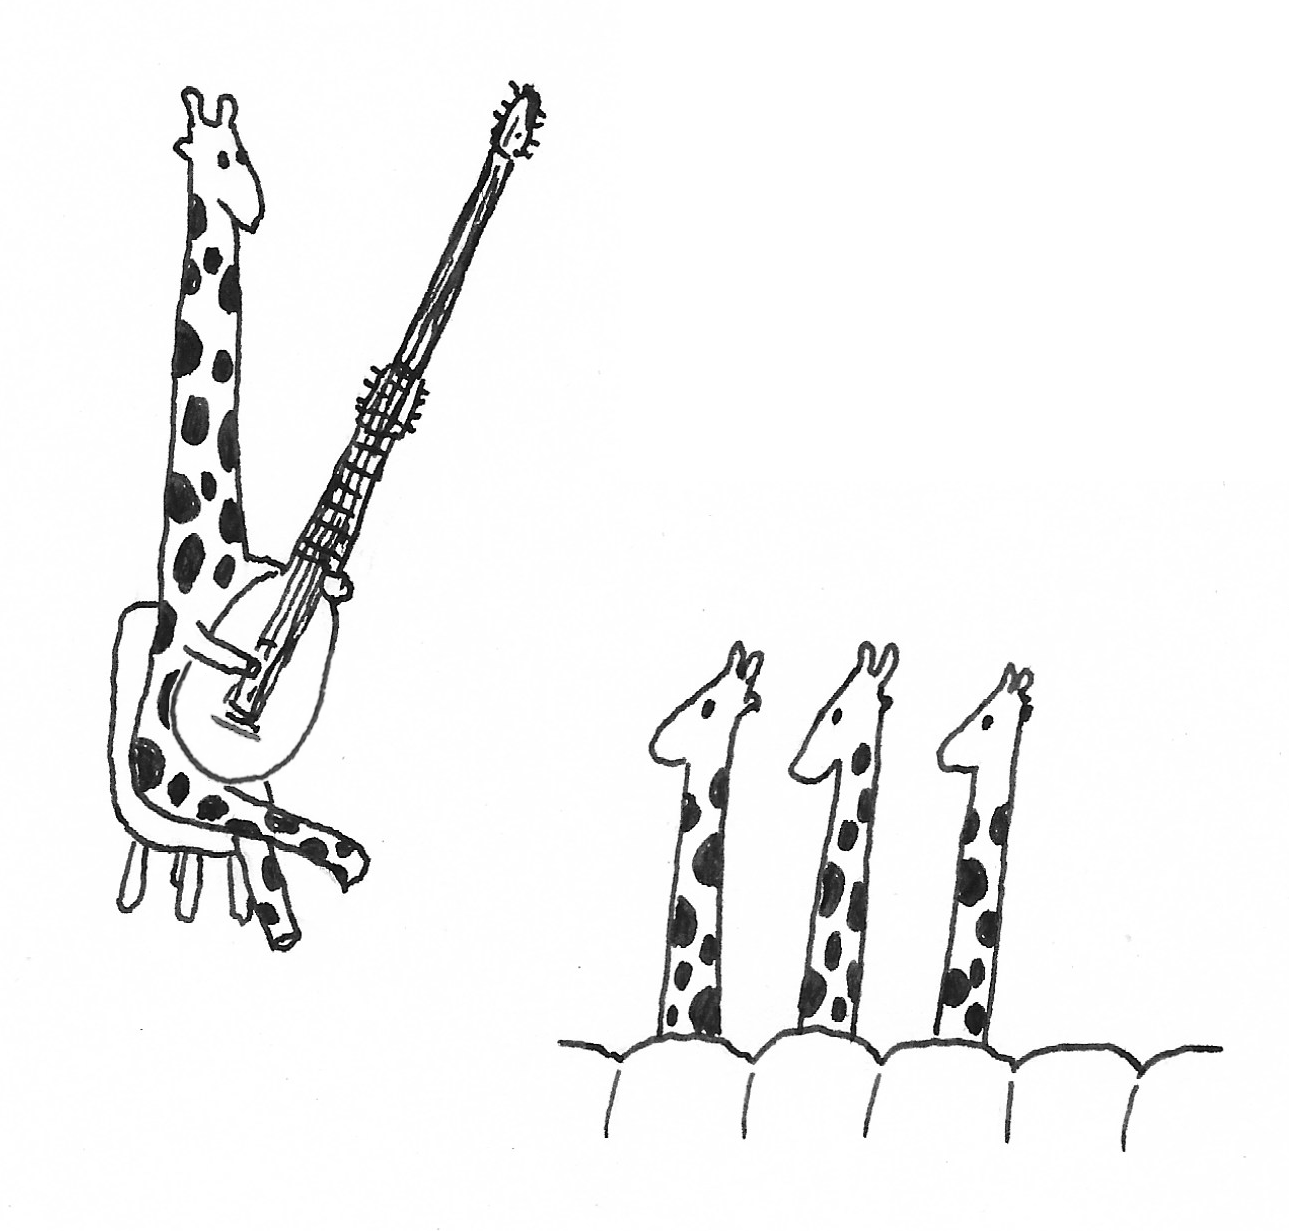
\includegraphics[width=0.7\columnwidth]{images/giraffe-archlute-2}
  \end{figure}
  
  \section{Future directions}

  We have identified three alternative directions for sustainable
  development, as follows.
  
  \subsection{``Enhanced ECOLM''}

  In this approach, we retain the relational data schema of the
  existing ECOLM, which is the only one of the datasets under
  consideration to have a formal schema, and provide ETL (extract,
  transform, load) data loaders for other sources. We then publish the
  schema, data dumps, and automation to rebuild or mirror the data,
  along with the code of our query interface and encourage others to
  attach their own interfaces or tools to it.

  Advantages of this approach include the ability to preserve existing
  code and to use original ECOLM records as a reference. The existing
  schema is detailed and fairly effective, provides appropriate
  structure, and reflects some good domain-specific
  decisions. Relational data import is a well understood field, and we
  could focus on user interfaces and data conversion rather than any
  novelty of data representation. If the work fails, the result should
  be at minimum a more open publication of the existing ECOLM.

  Disadvantages include that the schema has little in common with any
  of the ad-hoc solutions other maintainers have settled on, so all
  import and export would be custom. It also has little in common with
  wider current practice. The schema is perhaps already overspecified
  for its current use, yet does not address any problems relating to
  stable identifiers, versioning, or providing queryable APIs or data
  sources.

  Although we could at least initially reuse the existing user
  interface, it is no longer considered a strength of ECOLM and would
  need some work to update to modern expectations.

  \subsection{Graph-based}

  In this approach, we take the fundamental representation to be a
  graph of triples in the model of RDF, and convert all metadata to
  that for import and from it for query. External data such as
  transcriptions and multimedia resources are identified by
  graph-relatable identifiers such as URIs.

  Advantages include the use of a widely-understood and accepted model
  that meets common expectations about data compatibility and API
  provision. For schema we can draw ontologies from existing systems
  including the widely-used RISM. The structure is reasonably amenable
  to versioning and to use of ``idempotent'' import flows with
  automated testing, offering the option of ongoing import of changes
  in upstream sources. In principle existing tools may be used for
  review, query, inferencing, and conversion. The use of standard
  formats with automated tests could lead to a result far more easily
  maintained or mirrored by third parties.

  The approach has difficulties as well. It discards the existing user
  interface work and requires even the existing ECOLM data to be
  converted. Although graph representations have wide application,
  they are not generally used for manual data management and therefore
  have as little in common with the ad-hoc schemas of enthusiast lute
  resources as with that of ECOLM. Significant work would be required
  to maintain stable identifier mappings from external sources. With a
  more flexible structure than ECOLM's relational database, care and
  good automated testing would be needed to avoid ``silently missing
  data'' problems on query. Finally a separate solution would be
  needed to the problem of identifying and retrieving non-graph data
  such as media resources.

  Although in this approach we could no longer use the existing ECOLM
  user interface, that may be slightly mitigated by the ability to
  adapt other graph-driven UIs to the model.
  
  \subsection{``RISM-aligned''}

  In this approach, we concentrate on compatibility with formats and
  software used by RISM. The motivating principle is that RISM is the
  dominant ``entry point'' in this field and, although our sources are
  not all up to the standard indexed by RISM, we want to facilitate
  linkage for those that are, and to be prepared if in the future RISM
  should grow to cover the whole area of directly represented lute
  tablature. The ideal future here would involve replacing this
  project entirely with an aspect of RISM.

  In this approach the metadata representation might be
  MARC\footnote{https://www.loc.gov/marc/} (Machine Readable
  Cataloging) as it is within RISM, and possibly the RISM
  Muscat\footnote{https://rism.info/community/muscat.html} application
  might be used for management.

  \subsection{Summary}

  The three directions we have listed broadly correspond to common
  patterns in work of this type:

  \begin{enumerate}
  \item Choose one of the existing technical solutions already in use,
    and adapt the others to it;
  \item Adopt a higher-level ``linked data'' approach in which all
    existing resources are promoted to an interoperable format;
  \item Find an industry partner, adopt their tools, and contribute to
    their existing ecosystem.
  \end{enumerate}

  In this case RISM is the closest thing available to a
  standard-setting source of industrial tooling and integration, so it
  may serve as the equivalent of an industry partner. Hybrid
  approaches may also be practical, such as adapting the existing
  sources into a graph representation as a lowest-common-denominator
  precursor to conversion into other formats.
  
\end{sloppypar}
  
\end{document}
